%\pagestyle{plain} % No headers, just page numbers
%\pagenumbering{arabic} % Arabic numerals
%\setcounter{page}{1}

\chapter{\uppercase {Motivation and Methods}}
\label{ch:motivation}

The capability for PDT to generate and run on an unstructured mesh is important because it allows us to run problems without having to conform our mesh to the problem as much. The idea is to have a logically Cartesian grid (creating orthogonal ``subsets") with an unstructured mesh inside each subset. These logically Cartesian subdomains are obtained using cut planes in 3D and cut lines in 2D. Figure \ref{grid} demonstrates this functionality. It is decomposed into 3 subsets in x and 3 in y, with the first two subsets meshed using the Triangle Mesh Generator\cite{triangle}, a 2D mesh generator.

\bigskip

\noindent\begin{minipage}{\textwidth}
\centering
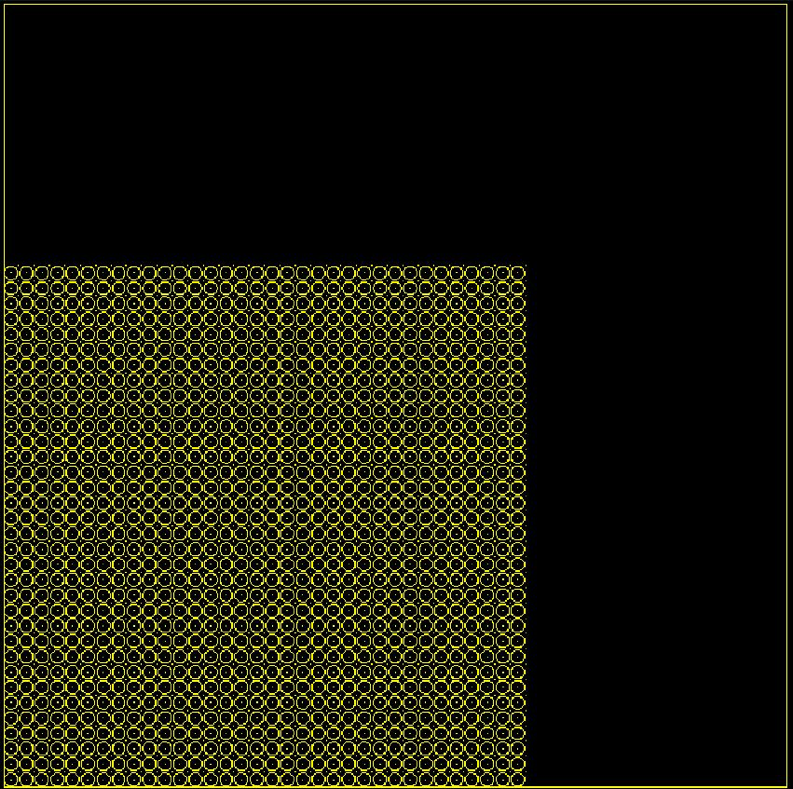
\includegraphics[scale = 0.5]{figures/lattice.png}
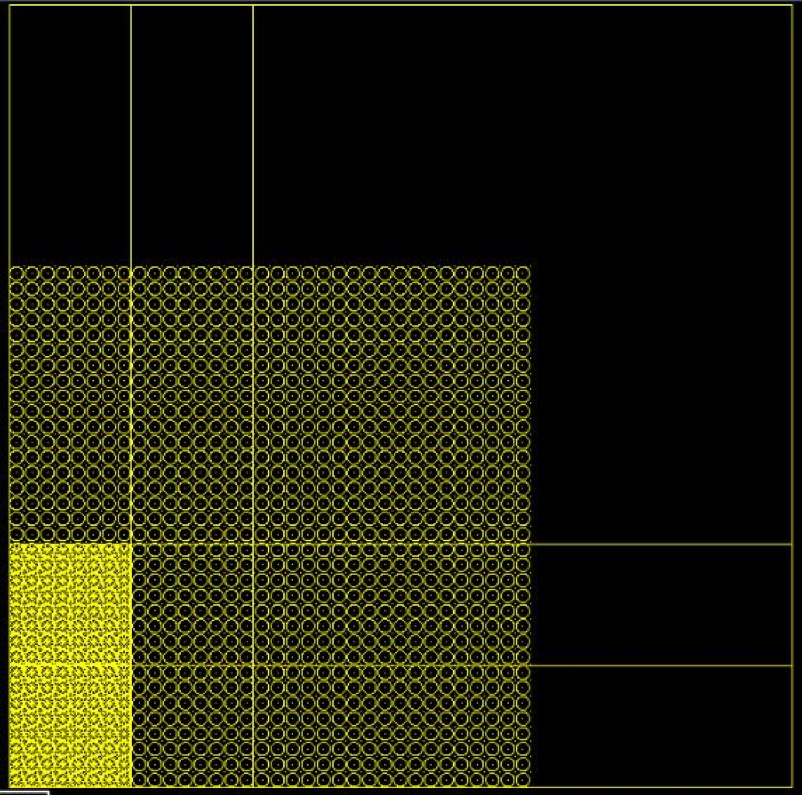
\includegraphics[scale = 0.5]{figures/subsetlattice.png}
\captionof{figure}{A PSLG describing a fuel lattice, and with a orthogonal ``subset" grid imposed on on the PSLG.}
\label{grid}
\end{minipage}
\smallskip

This orthogonal grid is superimposed and each subset is meshed in parallel.  Subsets are now the base structured unit when calculating our parallel efficiency. Discontinuities along the boundary are fixed by ``stitching'' hanging nodes, creating degenerate polygons along subset boundaries. Because PDT's spatial discretization employs Piece-Wise Linear Discontinuous (PWLD) finite element basis functions, there is no problem solving on degenerate polygons. 

When using the unstructured meshing capability in PDT, the input geometry is described by a Planar Straight Line Graph (PSLG). After superimposing the orthogonal grid, a PSLG is created for each subset, and meshed. Because the input's and each subset's PSLG must be described and meshed in 2D, the mesh can be extruded in the $z$ dimension in order to give us the capability to run on 3D problems. Obviously, this is not as good as an unstructured tetrahedral mesh, but for many problems, it is a great capability to have. 

When discussing the parallel scaling of transport sweeps, a load balanced problem is of great importance. A load balanced problem has an equal number of degrees of freedom per processor. Load balancing is important in order to minimize idle time for all processors by equally distributing (as much as possible) the work each processor has to do.  For the purposes of unstructured meshes in PDT, we are looking to ``balance'' the number of cells. Ideally, each processor will be responsible for an equal number of cells. 

If the number of cells in each subset can be reasonably balanced, then the problem is effectively load balanced. The Load Balance algorithm described below details how the subsets will be load balanced. In summary, the procedure of the algorithm involves moving the initially user specified $x$ and $y$ cut planes, re-meshing, and iterating until a reasonably load balanced problem is obtained.  Equation \ref{metric_def} shows the equation for calculating the load balancing metric, which dictates how balanced or unbalanced the problem is.
\begin{equation}
f =\frac{\underset{ij}{\text{max}}(N_{ij})}{\frac{N_{tot}}{I\cdot J}},
\label{metric_def}
\end{equation}
where $f$ is the load balance metric, $N_{ij}$ is the number of cells in subset $i,j$, $N_{tot}$ is the global number of cells in the problem, and $I$ and $J$ are the total number of in the $x$ and $y$ direction, respectively. The metric is a measure of the maximum number of cells per subset divided by the average number of cells per subset.

The load balancing algorithm moves cut planes based on two sub-metrics, $f_I$ and $f_J$. Equation ~\eqref{submetric} defines these two parameters:
\begin{align}
f_I &= \underset{i}{\text{max}}[\sum_{j} N_{ij}]/\frac{N_{tot}}{I} \notag \\
f_J &= \underset{j}{\text{max}}[\sum_{i} N_{ij}]/\frac{N_{tot}}{J}.
\label{submetric}
\end{align}

$f_I$ is calculated by taking the maximum number of cells per column and dividing it by the average number of cells per column. $f_j$ is calculated by taking the maximum number of cells per row and dividing it by the average number of cells per row. If these two numbers are greater than predefined tolerances, the cut lines in the respective directions are redistributed. Once redistribution and remeshing occur, a new metric is calculated. This iterative process occurs until a maximum number of iterations is reached, or until $f$ converges within the user defined tolerance. The Load Balance algorithm behaves as follows:

\lstinputlisting[language = C++, basicstyle = \footnotesize]{loadbalance.cc}

\noindent\begin{minipage}{\textwidth}
\textbf{Redistribute:} A function that moves cut lines in either X or Y. \\
\rule{\textwidth}{0.4pt}
\begin{algorithmic}
\STATE \textbf{Input:}CutLines (X or Y vector that stores cut lines). 
\STATE \textbf{Input:} num\_tri\_row or num\_tri\_col, a pArray containing number of triangles in each row or column 
\STATE \textbf{Input:} The total number of triangles in the domain, $N_{tot}$
\STATE stapl::array\_view num\_tri\_view, over num\_tri\_row/column
\STATE stapl::array\_vew offset\_view
\STATE stapl::partial\_sum(num\_tri\_view) \COMMENT {Perform prefix sum}
\COMMENT {We now have a cumulative distribution stored in offset\_view}
\FOR {$i = 1$ :CutLines.size()-1}

	\STATE vector $<$double$>$ pt1 = [CutLines(i-1), offset\_view(i-1)]
	\STATE vector $<$double$>$ pt2 = [CutLines(i), offset\_view(i)]
	\STATE ideal\_value = $i\cdot \frac{N_{tot}}{\text{CutLines.size()}-1}$
	\STATE X-intersect(pt1,pt2,ideal\_value) \COMMENT{Calculates the X-intersect of the line formed by pt1 and pt2 and the line y = ideal\_value.}
	\STATE CutLines(i) = X-intersect
\ENDFOR
\end{algorithmic}
\rule{\textwidth}{0.4pt}
\end{minipage} 

